\section{Approach}
%\BL{need more illustration about the reason why we introduce them in this order so that it's less confusing to readers}
Our overall approach is illustrated in \figref{fig:approach}.
Our starting point is a set of cross-lingual
named entities harvested from English and Chinese Wikipedia/Wikidata,
as well as a set of translation pairs of ordinary words from Bing translator API
(\secref{sec:vocab}).
These two sets serve as our vocabulary.
Then we conduct entity linking, of connecting named entities harvested with
text mentions
 in the English
and Chinese corpora
(\secref{sec:el}).
This step enables to understand named entities in the distributional semantic space, by creating English and Chinese word vector spaces respectively using skip-gram model, for both named entities an ordinary words.
Finally, in these two separate methods (\secref{sec:sim}),
we compute the cultural similarity scores
for each cross-lingual entity pair by either linearly transforming words
from the Chinese vector space into English or by merging the two spaces into
a new, higher-dimension translation space. Next, we explain each step in
more details.
%
%Firstly, we will talk about the vocabulary building. This preparation work helps us to determine the set of named entities that we want to study and  translation pairs. A translation pair consists of an English word and a Chinese word which share the same meaning.
%Entity linking is our second phase, in which we linked our interested named entities from plain text in order to distinguish their semantic meaning from common words.
%To construct the word-embedding vector spaces, we use the Skip-grams Model of word2vec to train our English and Chinese corpus.
%Finally, we will introduce cultural similarity computation, which is the core phase of our approach.
%
\begin{figure}[th]
\centering
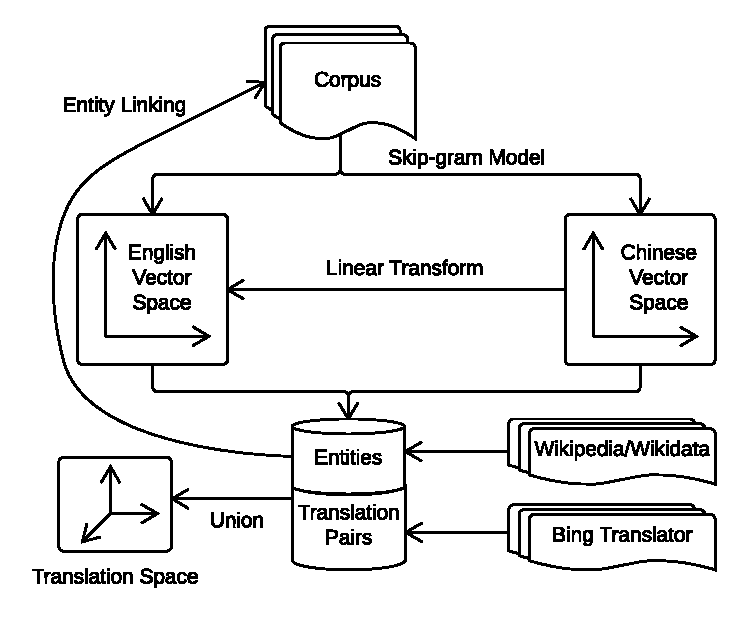
\epsfig{file=approach.eps, width=0.8\columnwidth}
\caption{Overall Workflow}
\label{fig:approach}
\end{figure}

%def: A translation consisting of an English word and its Chinese translation

%This section discusses the vocabulary, the method for entity linking, an overview of the
%Skip-grams model, which is the basis for capturing word semantics, as well as our
% two methods to compute cultural difference scores.

%\SH{we need to show a big picture, or overall architecture, after voca building as well. when/why we need linking}

\subsection{Vocabulary Building}
\label{sec:vocab}
%Vocabulary building is the very first step in our approach.
Our vocabulary has two parts: i) a set of named entities of interest
drawn from a standard ontology and ii) a set of ordinary English-Chinese
word pairs.
%Because we eventually are computing the similarity
%between English entities and Chinese entities, the entities and words
%from the two languages must be related by translation.
The obvious choice of this ontology is Wikipedia which keeps
an unique identifier for every documented named entity.
Many of these entities in Wikipedia have both English and Chinese instances and thus
make up the first part of the vocabulary.
%In addition, some English and Chinese pairs are connected by cross-lingual links.
%which make up first part of the vocabulary.
The ordinary words from
the two languages can be connected through online dictionary or translation APIs.
We discuss each step in further details below.
% together by normal word translation.

\subsubsection{Named Entities}

We focus on three categories of named entities, namely people, locations and
organizations.
%Ubiquitous ambiguities between English and Chinese makes
%a one-to-one correspondence crucial in a big range of inter-language tasks.
%We use the interlanguage links offered by Wikipedia to obtain pairs of
%named entity that exists both in English and Chinese Wikipedia.
%For instance, `Mao Zedong' is linked with its corresponding Chinese Wikipedia page. Therefore, we can generate entities pairs using inter-language linking based on its English name.
We ensure that an entity is a person if it belongs to the Wikipedia category
``Births by year''~\footnote{\url{https://en.wikipedia.org/wiki/Category:Births_by_year}}.
We consider an entity to be a location, if its Wikipedia page contains
longitude-latitude coordinates. An entity is considered as an organization,
if it appears under the subcategories of ``Organization'' in Wikidata while
it carries a Wikipedia page.
We use the interlanguage links offered by Wikipedia to make sure all named entity exist both in English and Chinese Wikipedia.



%
%\SH{this part may sound ad-hoc. maybe we'd better to very briefly mention, we leverage Wikidata, Wiipedia categories to mine all person, location, organization}
%
%We crawl all entities from all subcategories from . To get the list of locations, Wikipedia also gives us a great convenient. Wikipedia shows the coordinates of locations as \HY{(add a figure to show that)}. Therefore, we look through all English wiki pages with inter-language links and retain all entities with coordinate.
%For the organization list, the category on the Wikipedia is quite complicated and difficult to follow through a whole list of entities, so we turn to the freely available knowledge base based on Wikipedia, Wikidata. It has a class called ``Organization''\footnote{\url{https://www.wikidata.org/wiki/Q43229}}, and we recursively queried all the entities which are an instance of this class or an instance of the sub-classes of ``Organization'', while possessing both an English Wikipedia page as well as a Chinese Wikipedia page, using the web interface\footnote{\url{https://query.wikidata.org/}} with SPARQL. Finally, we manually check our list and filter out some unreasonable entities.
%

\subsubsection{Translation Pairs}

%Since it is a bilingual problem, we have to construct a bridge between English and Chinese, so that not only those named entities discussed earlier have their pairs, but also the common words in both corpus. However, normal words are slightly different between English and Chinese.
%For English, we lemmatize words except named entities. We have all lemma and then we set a threshold to filter out less frequent lemma. For Chinese, we similarly set a threshold. But instead of lemmatization, we apply a word segmentation tool \HY{(which tool?)} to the text.
%\HY{(how to do intersection for translation and vocabulary?)}
%
%\SH{to NLP people, this part may seem trivial= using dictionary to generate many-to-many mapping. we can explain why we use Bing and highlight only the difference}
%
%Translation between English and Chinese is a many-to-many mapping.
%\figref{fig:translation} shows an example of the many-to-many translation mappings, where an English word may have more than one suitable Chinese word translations, and a Chinese word can be translated from more than one English words.
To construct the set of translation pairs of ordinary words, we first collect common
English words from a large lemmatized English corpus and translate
these words into Chinese translations using online
dictionary and translation APIs,
specifically Bing
API~\footnote{\url{http://www.bing.com/translator}} in this work. As each English word can be translated into multiple Chinese words, and a Chinese into multiple English words, this phase generates
a many-to-many translation mapping.
%as shown in \figref{fig:translation}.

%we queried and crawled every word with more than 50 occurrences in our lemmatized English corpus in  to get all translation pairs between English and Chinese as our common word dictionary.
%\begin{figure}[th]
%	\centering
%	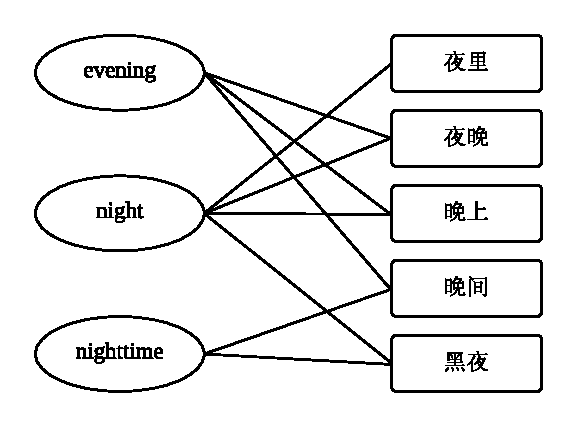
\epsfig{file=translation_pair.eps, width=0.7\columnwidth}
%	\caption{An example of the many-to-many translation pairs}
%	\label{fig:translation}
%\end{figure}

\subsection{Entity Linking}
\label{sec:el}

The purpose of entity linking is to link mentions of entities of
our interest in a large text corpus to our vocabulary.
This enables to project a named entity in the distributional semantic space,
together with ordinary words.

However, this step is tricky, as the same entity is represented as many
surface forms:
 For example,
both ``William Jefferson Clinton'' and ``Clinton'' may refer to entity
``Bill Clinton'' while ``Clinton'' may also refer to ``Hillary Clinton.''
Though entity linking has been actively studied to address this problem, we could not
adopt existing solution ``as is", due to the following two reasons:
First, pursuing the balance of precision and recall, they tend to generate too many links
for our task requiring high precision.
Second, existing approaches building on linguistic signals cannot apply equally to English and Chinese entity linking.

We devise a simple alternative achieving the comparable precision target.
We obtain the set of possible surface forms for an entity by
collecting all anchor texts of the entity in the Wikipedia corpus.
%Our job here is to link anchors in the text to corresponding entities.
In addition, we leverage a redirect system of Wikipedia,
%Wikipedia has a redirect system. The entity ``UK'' is
redirecting ``UK'' to ``United Kingdom'' in Wikipedia.
We merge all entities that redirect to each other as one entity.
We can also compute anchor-entity linking frequency from
the Wikipedia corpus.

Our entity linking algorithm starts by looking for potential anchors
in the plain text corpus. We adopt a longest match strategy here that
prefers longer anchors. This is because we assume
longer anchors are more reliable and bring about higher precision.
In Entity linking, we aim for high precision rather than recall because
even if an entity is not recognized in the text, its constituent words
will still be captured later in the ordinary word vector space and
contribute to the semantics of other entities or words.
%Therefore, we enumerate substring of tokens from longest to
%shortest and try to find links for them based on the following rules.
%We consider text article by article.

For a recognized anchor $a$ in the plain text,
typically this string has been linked to multiple
entities in Wikipedia pages before. All these linked entities are considered
candidates $C$ for linking $a$ presently.
We conduct the following checks to select an entity in $C$ to link.
First, if $a$ is identical to the Wikipedia title of some entity
$e \in C$, then we directly link $a$ to $e$.
Second, if $e \in C$ has already been linked to another anchor in
the current text, then we link $a$ to $e$. If multiple $e$ in $C$ have been
linked already in the text, pick the nearest one in the text.
Otherwise, we link $a$ to an $e$ in $C$ if $e$ satisfying
three conditions:
\begin{align}
\frac{freq(a, e)}{\sum_{c_i \in C}freq(a, c_i)} &> 0.5\\
freq(a, e) &\geq 5\\
|C| &\leq 5
\end{align}
where $freq(a, e)$ is the number of times $a$ is linked to $e$ in
Wikipedia corpus. The first condition holds
when $e$ is a dominant sense (link) for $a$,
which means there is a high prior probability that $e$ is the right
entity for $a$. The second condition
ensures that $a$ links to $e$ considerable number of times in Wikipedia,
which filter out mistakes by editors and rare anchors.
The last condition is designed for anchors that are highly ambiguous.
For example, most of the time, ``Singh'' refer to ``Manmohan Singh'' in
Wikipedia, the former Prime Minister of India, we can not
confidently link ``Singh'' to ``Manmohan Singh'' when we first see
the anchor ``Singh'' in a plain text article because ``Singh'' is
a very common Indian name that can be linked to many entities.
But if there is already an anchor that links to
``Manmohan Singh'' in the same article,
the confidence is much higher. In practice, the above heuristics
have been shown to significantly enhance the precision of entity linking.

\subsection{Skip-gram Model}
\label{sec:skip}

Entity linking enables us to adopt
 Skip-gram model introduced by Mikolov
et al.~\shortcite{Mikolov2013distributed}
to train word embeddings to include both named entities and ordinary words,
 from English and Chinese corpus separately.
After this step, two vector representations are generated
for every word from English and Chinese vocabulary.
Note that both ordinary words and entities are considered ``words''
here.

Skip-gram is an unsupervised learning model where the basic idea
is to predict co-occurring words in a corpus.
%In the Skip-gram model, the objective is to maximize the average
%log probability
%\begin{equation}
%\frac{1}{T} \sum_{t=1}^{T} \sum_{j=-c}^{c} \log p(w_{t+j}|w_t),
%\end{equation}
%where $c$ is the size of training window,
%and $T$ is the total size of training corpus.
%$p(w_i|w_j)$ is defined by a softmax function
%\begin{equation}
%p(w_i|w_j)=\frac{\exp(u_{w_i}^{\top} v_{w_j})}{\sum_{l = 1}^{V} \exp(u_l^{\top} v_{w_j})},
%\end{equation}
%where $V$ is the size of the vocabulary, $u_w$ and $v_w$ are
%the ``input'' and ``output'' vectors representing the word $w$.

In our experiments, we set the window size as 5
and the size of ``input'' and ``output'' vectors to 150.
Further we discard any word that occurs less than 5 times in the whole corpus
and use negative sampling.

After we train this model on each monolingual corpus,
vector representations are generated for every word and every entity
from our vocabulary. We thus have two vector spaces:
one for English corpus and the other for Chinese corpus.

\subsection{Cultural Similarity Computation}
\label{sec:sim}
Next we introduce two algorithms for computing cultural similarity between
the English vector and the Chinese vector of the same entity. The
cultural difference can then be readily induced from the similarity.
%The inverse of the similarity between the vector representations
%for corresponding English and Chinese gives the amount of cultural difference for a pair.

\subsubsection{Linear-transformation Algorithm}

%\SH{since this idea is originated from Mikolov,
%can we state the similarity/difference early on? why we need a new method?}

English and Chinese vector spaces trained from the Skip-gram model
are not directly comparable due to unknown meaning of each dimension.
However, Mikolov et al. \shortcite{Mikolov:2013tp} have shown that
the relationship between these vector spaces can be captured by
rotation and scaling, represented by a linear transformation matrix $W$.
In this paper, we borrow this idea and train this matrix
using a number of human annotated ``seed entities" with {\em little}
cultural difference and using the following optimization problem:

\begin{equation}
\argmin_{W}\sum_{i=1}^{n} || Wx_{i}-t_{i} ||^2,
\end{equation}
where $x_{i}$ is a word in Chinese while $t_{i}$ is its
corresponding translation in English and $n$ is the size of
training samples.

Thus we train a linear transformation matrix from Chinese to English spaces and map each Chinese word vector to the English space.
This transform enables to visualize English and Chinese vectors in the same coordinate.
% as illustrated in
%Finally we calculate the cosine similarity between the two vectors in the English space.
\figref{fig:embeddingspace} shows an illustrative example
of how we linearly transformed the embedding space of one language
to match with that of another language.
This example shows that, after the transformation,
both Chinese and English word vectors are in the same coordinate,
while the angle between Chinese and English version of ``Dalai Lama''
is larger than that between Chinese and English version of ``Roger Federer''.
This suggests that Dalai Lama, a controversial political figure,
has a larger cultural difference in Chinese and English, than Roger Federer,
a famous tennis player.

\begin{figure}
	\centering
	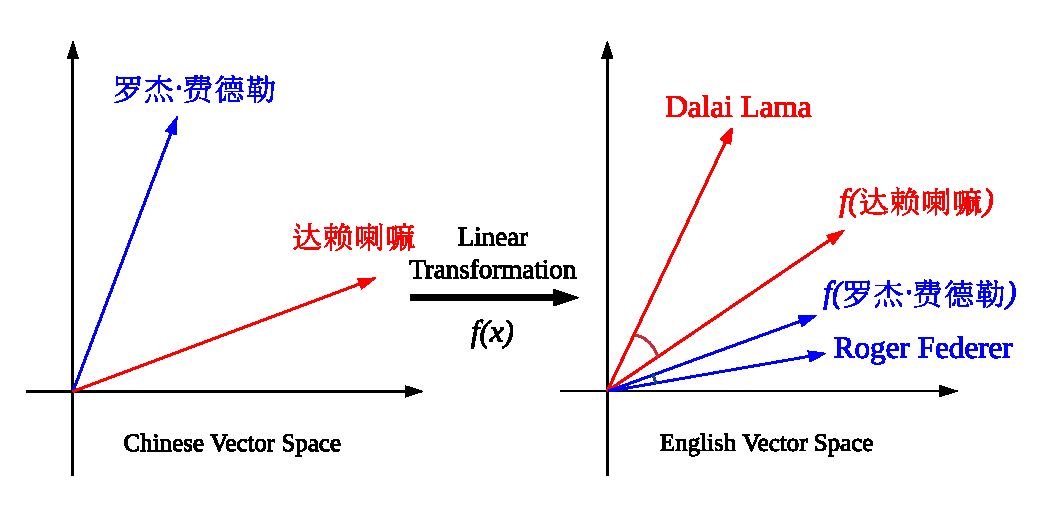
\epsfig{file=embedding_space.eps, width=0.9\columnwidth}
	\caption{Linear transformation from Chinese to English}
	\label{fig:embeddingspace}
\end{figure}


Despite the power of linear transformation, its performance strongly
depends on the quality of the seed entities.
However, obtaining high quality seed entities requires time and bilingual annotators.
We thus propose an alternative unsupervised approach, called \emph{translation space algorithm}.

%Sometimes creating a good
%set of seed entities may not be a great idea due to the limited
%time and resources. Therefore, we further propose an unsupervised
%method called translation space algorithm.

\subsubsection{Translation Space Algorithm}

This section combines English and Chinese semantic spaces into
a rich and higher dimensional space , leveraging many-to-many translation pairs
created in \secref{sec:vocab}.

Specifically, %In this method,
we first represent each entity in a word vector space
by its cosine similarity with all words or entities in the
same space, including itself.
%we can obtain {\em distance vector} of term $w_i$,
%where $j^{th}$ dimension for the distance
%vector represents the distance to word $w_j$ in the vocabulary.
%in order to get an $n$-dimensional vector, where $n$ is the total number of
%terms in our vocabulary. We call this $n$-dimensional vector {\em distance vector},
%and the $i^{th}$ dimension for the distance
%vector represents the distance to word $w_i$ in the vocabulary.
%For $i^{th}$ named entity, we call distance vector from English corpus $D_{EN, i}$. Therefore,
Suppose we want to compute the cultural similarity score for a pair of
entities $w_e$ and $w_c$ in the English and Chinese vector spaces respectively.
We first represent $w_e$ by a
{\em similarity vector} of size $l_e$ where $l_e$ is the total number of
words/entities in the English space, and each dimension of this
vector is the cosine similarity between $w_e$ and all words in English.
The cosine between $w_e$ and itself is 1.
We represent $w_c$ similarly. Because the English and Chinese vocabularies
are of different sizes, these two similarity vectors are of different sizes,
too. Furthermore, since the translation is many to many,
the two vectors are not directly comparable.

Our solution is to ``expand'' these two vector spaces in a higher dimensional space,
where each dimension represents a translation from one English word
to the corresponding Chinese word. As such, the new space, known as the
``translation space'', is $k$-dimensional, where $k$ is equal to the total
number of translation pairs or edges between the two vocabularies.
In \figref{fig:transspace}, as an example,
consider a word $x$ in the similarity
vector of $w_e$. If $x$ is translated to $y$ and $z$ in Chinese,
without prior information, we assume $x$ is translated to $y$ and $z$ with
equal probability. As a result, the dimension for $x$ is then
expanded into two new dimensions,
namely $xy$ and $xz$, where each dimension stores the same value
as the value for $x$.

\begin{figure}[th]
\centering
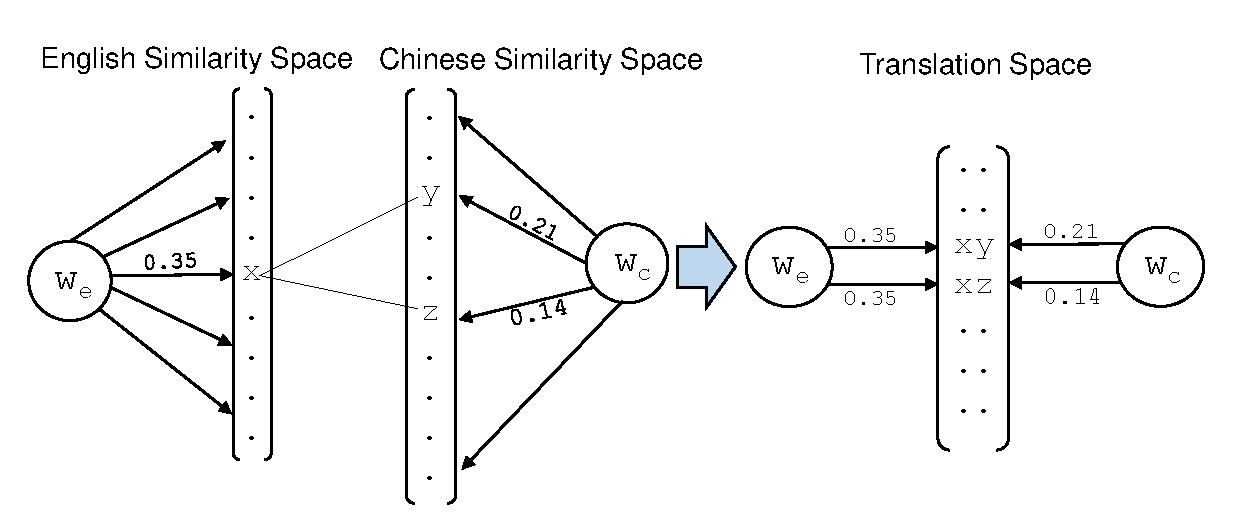
\epsfig{file=vector.eps, width=1.1\columnwidth}
\caption{Example for Translation Space Algorithm}
\label{fig:transspace}
\end{figure}

%entity $w_i$ in English space is
%denoted as $D_{EN, i}$, and its $j^{th}$ dimension is
%\begin{equation}
%D_{EN, i, j} = cos(v_i, v_j)
%\end{equation}
%where $v_i, v_j$ are the embeddings for $w_i, w_j$ respectively.
%We can create a similarity vector $D_{CH, i}$
%for the same entity in Chinese corpus.
%
%If there is a one to one mapping between each dimension from
%English space and Chinese space, these two similarity vectors are
%directly comparable.  However, as we mentioned previously,
%the translation mapping is many to many.
%Without loss of generality, we assume here that a word $w_j$ maybe translated
%to all its translations with equality probability. Thus we can split
%dimension representing word $w_j$ into $s$ dimensions where $s$
%is the number of translations for $w_j$.
%We set the value of these dimensions to the same value
%as the distance to $w$. That is to say, we build two new distance vectors in translation
%pair level. We call them $D'_{EN, i}$ and $D'_{CH, i}$. If $j^{th}$ pair of translation
%is $(w_{EN, k}, w_{CH, l})$ where $w_{EN, k}$ is $k^{th}$ term in English vocabulary
%and $w_{CH, l}$ is $l^{th}$ term in Chinese vocabulary, we have
%\begin{equation}
%D'_{EN, i, j} = D_{EN, i, k}
%\end{equation}
%\begin{equation}
%D'_{CH, i, j} = D_{CH, i, l}
%\end{equation}

At this point, the similarity vectors of $w_e$ and $w_c$
are mapped to the new translation space and are now comparable.
Now we can calculate the cosine similarity between $w_e$ and $w_c$
pairs in the translation space as the cultural similarity score
between the two entities.

%\subsubsection{KNN-set Algorithm}
%
%Followed the same idea as distance-vector algorithm and famous K-nearest-neighbors
%algorithm. We split all words according to its translation. \HY{Plz improve the following statement}
%Therefore, for each pair of English and Chinese terms, we can find $k$ nearest neighbors
%for both the Chinese and English word in their respective embedding space.
%Here we use cosine similarity as distance metric to find $k$ nearst neighbors.
%In our experiment, we tune $k$ to be \HY{100?}100. Once we have these neighbors, we can use
%this set of terms to represent the orginal English or Chinese term.
%Since each element from two sets represents a translation between Chinese and English terms,
%we can map the neighbors in the Chinese set to English and calculate
%Jaccard similarity between this mapped set and original English set as follows:
%
%\begin{equation}
%J(A,B)=\frac{|A \cap B|}{|A \cup B|}
%\end{equation}
%where $A$ and $B$ are two sets.
